\documentclass[11pt]{article}
\usepackage[latin1,utf8x]{inputenc}
\usepackage{color}
\usepackage[pdftex]{graphicx}
\usepackage{amsmath, amsfonts, amssymb, amsthm}



\title{Titolo da decidere}
\author{authors}
\date{date}
\begin{document}
\maketitle
\begin{abstract}
This is a very short abstract.
\end{abstract}

\section{Introduction}

\textcolor{blue}{
Process mining is a recent discipline that includes tecniques for process analysis and discovery. Today, many Information Systems that integrate the concept of business process, provide registration of events that occur during the execution of the process activities. Starting from recorded executions related on the same process, the goal of the existing process mining techniques is extracting data to discover automatically a process model or, if the model is already exists, to check the executions in term of conformance and performance.\\
\newline
The idea that ispires this work consists in developing un approach for exploiting the huge ammount of data recorded at the process activities by information systems. More precisely, our purpose is to find pattern on data that could influence the process behaviour. For this reason, the work presented in this article is based on some concepts originated to Machine Learning and Data Mining disciplines. Should be noted that using data mining for similar aims has already been explored by Van der Aalst in \cite{}, the idea here consists in discovering how data attributes may influence the routing of case. Instead, in this contribution the intention is to present an approach based on data mining techniques also, but for discovering data dependencies on the process conformance and performance. Finally, an another goal that we propose is providing a predective model to detect the conformance result and some performance metrics for new process executions.  \\}
\newline
\textcolor{blue}{In front of a very large number of process instances, all recorded in event log, it is essential to have an automatic tool for extracting usefull information for the analysis of the real behaviour of the process. In order to meet this requirement, in this article we present an approach based on classification and decision trees to identify rules that could influence the process in term of conformance to the existing model, and performance metrics.\\}
%\newline
%\textcolor{blue}{
%}

%Il process mining comprende una serie di tecniche che trattano processi vigenti in contesti organizzativi. Attualmente, moltissimi sistemi che integrano il concetto di processo di business a loro interno, provvedono alla registrazione degli eventi che si verificano durante l'esecuzione delle attività previste dal processo. Partendo da un insieme di esecuzioni registrate e riguardanti un unico processo, è possibile applicare una serie di tecniche volte alla scoperta del modello di processo oppure alla sua analisi in termini di conformance e performance. L'idea che ispira questo articolo è sviluppare un approccio in grado di sfruttare le enormi quantità di dati che vengono registrati in corrispondenza delle varie attività del processo.
%Si tratta di un approccio basato sulle tecniche di data mining capace di scoprire eventuali influenze dei dati sul comportamento del processo. L'impiego del data mining per il process mining è un'idea già presentata da Van deer Aalst in \cite{}, in questo articolo infatti si cerca di evidenziare le influenze dei dati sulla direzione del flusso di esecuzione in corrispondenza dei punti decisionali. La nostra idea invece è di sfruttare le tecniche di data mining per fornire agli analisti di porcesso un tool di supporto in grado di aiutare nell'analisi di conformance e performance del processo.\\




%Di fronte ad un numero molto grande di istanze di processo, tutte appositamente registrate in event log, avere uno strumento capace di estrarre informazioni utili per l'analisi del comportamento reale del processo diventa fondamentale. Cercando di rispondere a questa esigenza, in questo articolo è presentato un approccio capace di individuare eventuali regole che influenzano il processo in termini di conformance al modello prefissato, ed in termini di performance. Un ulteriore obiettivo che ci poniamo è fornire agli analisti uno strumento di predizione, ovvero un modello in grado di predire, in base ai dati delle nuove istanze di processo che si presentano, quale sarà l'esito di conformance e le misure di performance che caratterizzano la particolare esecuzione presa in esame. Per potere realizzare questi obiettivi ci basiamo sulla classificazione che è una particolare tecnica di data mining, vengono inoltre impiegati gli alberi di decisione come strumento di classificazione.\\


%L'articolo è organizzato in questo modo: dopo una presentazione nella sezione 2 dei vari formalismi adottati, nella sezione 3 viene presentato un semplice esempio a cui verrà fatto riferimento nell'articolo. Nella sezione 4 invece verranno introdotti alcuni concetti relativi alla conformance e performance di un processo. Infine, nella sezioni 5 e 6 si affronterà come impiegare la tecnica di classificazione per scoprire particolari pattern nei dati che possono influenzare conformance e performance del processo.

\textcolor{blue}{
The article is organized as follows. After an introduction to the different formalism used to carry out our purposes, the attention will be...
}

\section{Example}\label{example}


\begin{figure}[t]\label{ConfLog}
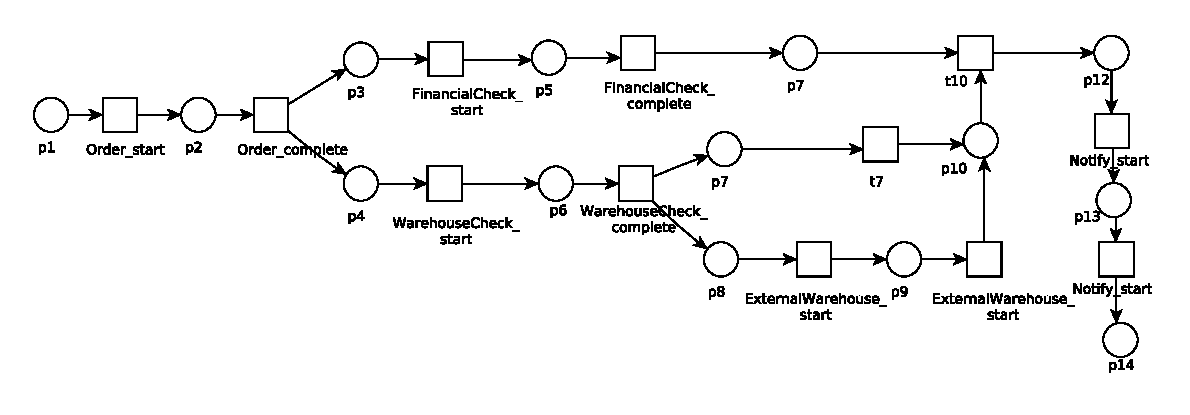
\includegraphics[width=360pt]
{./items/Sales_PN.pdf}
\caption{Petri net}
\end{figure}

L'esmepio scelto si ispira ad una procedura che trova applicazione all'interno di organizzazioni a carattere commerciale, si tratta del processo di vendita. In questa sede viene considerata solo una sua semplificazione rispetto a quanto avviene realmente. Per noi, il processo di vendita inizia con l'attività 'notify', in questa fase viene accolto un ordine da parte di un cliente. Dopo la ricezione dell'ordine, vengono condotte alcune attività in parallelo (visto che non presentano alcuna dipendenza tra loro) una di queste è l'attività 'FinancialCheck', in questa fase viene effettuata una valutazione dell'ordine dal punto di vista finanziario, possiamo ad esmepio pensare che vengono condotte delle indagini sulla solvibilità del cliente che ha emesso l'ordine. Parallelamente viene svolta l'attività 'ExternalWarehouse'...

\section{Conformance and Performance Analysis based on Petri nets}

The process analysis is performed by using the Petri net modelling the process and an event log recording the related executions (process instances). The basic building blocks of event logs are events. An event {\itshape e} can be seen as a pair {\itshape e = (a,t) } representing an action {\itshape a } recorded and the corresonding timestamp {\itshape t}. Action and timestamp are denoted respectively by $\alpha(e)$ and $\phi(e)$. Events that belong to the same process are grouped into {\itshape traces}. Formally, a trace $T$ is a finite sequence of events $T[1],..., T[n]$, such that $\phi(T[i]) \leq \phi(T[i+1])$ for all  $i \in [1,n)$. A log $L$ is a set of traces, recording the activities performed by a system during a finite number of process executions. We assume here the following hypothesis:
\begin{itemize}
\item All traces are instances of the same process.
\item For each action there exists a corresponding transition in the net that will be denoted, for simplicity, by the same name of the action.
\end{itemize}
The key algorithm expoloited to analyze the Petri net model with respect to the log is the {\itshape log repaly} algorithm. Given a Petri net model and an event log as intput to the algorithm, the output results can be used to check the conformance of traces and to evaluate some performance metrics. For each trace in the log, log replay starts by placing one token in the start place of the net. For each event in the trace the corresponding transition is fires in an {\itshape non blockin way} and the marking of the net is updated. ``Non blocking replay'' means that if the log replay execution requires to fire an enabled transition, the missing tokens are created artificially. The output of the log replay of a trace can be represented as an orderd list $R$ of pairs $(tr, i)$, representing that the transition $tr$ has been fired to mimic the event $T[i]$.
\\

In general, there could be exist some transition in the net called {\itshape invisible}. This can happen if the transition models an internal choice that is not visible in the system, or it is used to implement a construct of a more abstract modelling language (BPMN or others). Usually, invisible transitions are considered to be lazy, i.e, when firing a visible transition $t$ corrisponding to an event of the trace, only then the invisibile transition enabling $t$ is fired. However, in this paper, we adopt an other way for handling these transitions and the firing is performed as soon as possible. This allows to carry out some performance measures as explained that are not possible with the lazy metohode as explained in \cite.(riferimento al paper Applying Process Analysis to the italian eGiv Entreprise Architecture)\\

The result of log repaly can be used to evaluate conformance and performance of the Petri net model. Conformance problems can be discovered by analyzing the tokens that have been artificially created {\itshape (the missing tokens)} and the tokens tha were not consumed {\itshape (the remaining tokens)}.\\

To clarify the conformance analysis technique we exploit the Petri net presented in section \ref{example} with reference to tow traces , $T$ and $T'$, presented respectively in figures \ref{ConfLog} and \ref{NonConfLog}. The log replay execution of the trace $T$, which is compliant with the Petri net, terminates with a marking containing one token in the end place \{${p14 \rightarrow 1}$\}, and returns the sequence:
\begin{equation}
\begin{split}
R&=\{(Order\_start,1), (Order\_complete,2),(WarehouseCheck\_start,3), \\
& (FinancialCheck\_start,4),(WarehouseCheck\_complete,5),\\
& (FinancialCheck\_complete,6),(t10, 6), (Notify\_start,7), (Notify\_complete,8)\}
\end{split}
\end{equation}
The log replay execution of the trace $T'$ terminates with remaing tokens \{${p8 \rightarrow 1,p14 \rightarrow 1}$\} and a missing token \{${p10 \rightarrow 1}$\}. The missing token is created artificially and this fact records a wrong execution of the event $Notify\_start$. In fact, notice that in the trace $T'$ this event is executed before the termination of the activity ``FinancialCheck'', and this is interpreted as a non conformance to the process model. The sequence returned by log replay is:
\begin{equation}
\begin{split}
R'&=\{(Order\_start,1), (Order\_complete,2), (WarehouseCheck\_start), \\
& (FinancialCheck\_start,3), (WarehouseCheck\_start,4),(t7,5), (t10,6)\\
& (Notify\_start,6), (Notify\_complete,7)\}
\end{split}
\end{equation}

\begin{figure}[t]\label{ConfLog}
\centering
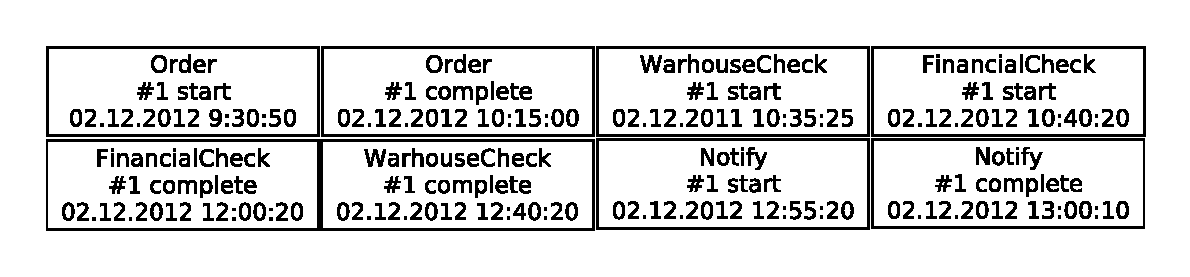
\includegraphics[width=400pt,height=40pt]
{./items/logConforme.pdf}
\caption{Conforme log example}
\end{figure}

\begin{figure}[t]\label{NonConfLog}
\centering
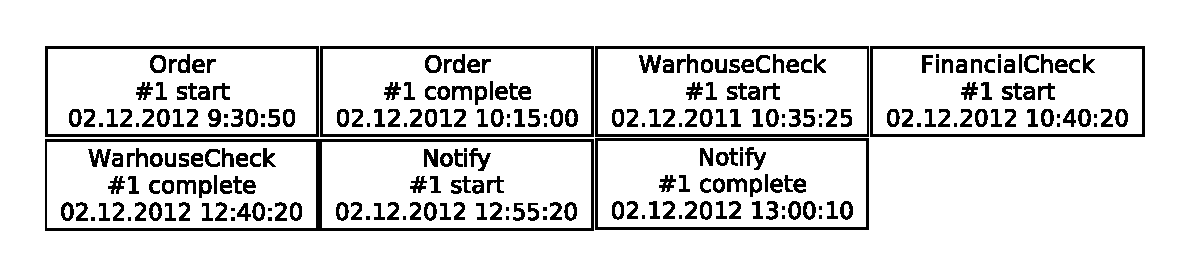
\includegraphics[width=400pt,height=40pt]
{./items/logNonConforme.pdf}
\caption{Non conforme log example}
\end{figure}

Since the logs contain timestamps, the log replay can be used to compute performance measures of the process. The idea is to calculate the time interval between production and consumption of tokens in each place. This tecniques can be applied only to traces that do not present missing token during the replay, because such tokens cannot have time information. During the log replay the following metrics can be computed for catch trace and each place:
\begin{itemize}
\item sejour time $(tsj)$ : the time interval between arrival and depature of tokens;
\item synchronization time $(tsc)$: the time interval between arrival of a token in the place and enabling of a transition in the post-set of the place;
\item waiting time $(tw)$:  the time interval between enabling of a transition in the post-set of the place and token departure (thus $tsj=tsc+tw $).
\end{itemize}

To clarify the metrics evaluated by this tecnique, as done with conformance analysis, we exploit the Petri net  presented in section \ref{example} and the trace T presented in figure \ref{ConfLog}. The replay starts with firing the transition $Order\_start$ at time $0s$, thus a token arrives at $p2$ at time $0s$. After $45 min$ the token in $p2$ is consumed and the transition $Order\_complete$ is fired, so $tw(p2)=tsj(p2)=45min$, and a token arrives at $p3$ and $p4$. At the time $1h:5min:25s$ the transition $WarhouseCheck\_start$ is fired, thus $tw(p4)=20min+25sec$ and a token is produced at $p6$. At the time $1h:10min:20s$ the transition $FinancialCheck\_start$ is fired and a token is produced at $p5$, so $tw(p3)=25min+20s$. After $2h:30min:20s$ from the replay start the transition $Financial\_complete$ is fired, hence we have $tw(p5)=1h+20min$ and a token is produced at $p11$. At time $3h:10min:20s$ the firing of the transition $WarehouseCheck\_complete$ is executed, so $tw(p6)=2h+4min+55s$ and token is produced at $p7$ and $p8$. At the same time the invisible transition $t10$ is fired and a token is produced at $p10$. At this point the transition $t10$ is enabled, so firing it is now possible and a token is produced at $p12$. Notice that $tsc(p11)=40min, tsc(p10)=0s$. At the time $3h:25min:20s$ the transition $Notify\_start$ is fired and a token is produced in $p13$, after $4min+4sec$ the trasition $Notify\_complete$ is fired and $tw(p13) = 4min+40s$.


\end {document}
